\section{Solutions to Chapter~\ref{chap-extension-trans-fourier}}

\begin{correction}{exo-eigenvectors-transfo-hartley}
Since $\Hh^2=N\Id$ and $\Hh$ is real symmetric, its possible eigenvalues
are $\pm\sqrt N$. For $V=\Hh/\sqrt N$, the orthogonal projectors are
\[
 P_+=\tfrac12(\Id+V),\qquad P_-=\tfrac12(\Id-V).
\]
They satisfy $P_++P_-=\Id$, $P_+P_-=0$, and $VP_\pm=\pm P_\pm$.
Thus a nonzero $P_\pm f$ is an eigenvector; zero projections must be
discarded. Choosing $\log(-1)=\imath\pi$ gives
\[
 V^t=P_++e^{\imath\pi t}P_-,\qquad
 \Hh^t=N^{t/2}V^t.
\]
The family $V^t$ is unitary for real $t$, satisfies
$V^{s+t}=V^sV^t$, and starts at the identity. The unnormalized powers have
the additional factor $N^{t/2}$. Program~\ref{listing-transfo-hartley-interm}
computes the unitary version used in the figure.
\begin{listing}[H]
\PythonCode{listing-transfo-hartley-interm}
\caption{Unitary fractional powers of the normalized Hartley transform.}
\label{listing-transfo-hartley-interm}
\end{listing}
\end{correction}

\begin{correction}{exo-transfo-hartley-generalisee}
Let $C_{nk}=\cos(2\pi nk/N)$ and $S_{nk}=\sin(2\pi nk/N)$, and let
$Jf=f^\sharp$. Root-of-unity sums give
\[
 C^2=\tfrac N2(\Id+J),\quad S^2=\tfrac N2(\Id-J),\quad CS=SC=0.
\]
Now $\Hh_\lambda=\cos\lambda\,C-\sin\lambda\,S$, so
\[
 \Hh_\lambda\Hh_{\pi/2-\lambda}
 =\sin\lambda\cos\lambda(C^2+S^2)
 =\tfrac N2\sin(2\lambda)\Id.
\]
This proves the inverse formula, including the factor $1/N$. If
$\sin\lambda=0$, the antisymmetric subspace is annihilated; if
$\cos\lambda=0$, the symmetric subspace is annihilated. Both subspaces
are nonzero for $N\geq3$, proving the stated necessity as well.
\end{correction}

\begin{correction}{exo-interpolation-transfo-hartley}
Write $N=2K+1$ and $g=\Hh(f)$, with indices interpreted modulo $N$.
The interpolant is
\[
 F(x)=\frac1N\sum_{k=-K}^{K}g[k\bmod N]\cas\frac{2\pi kx}{N}.
\]
At integer $x$, the inversion identity gives $F(x)=f[x]$. The use of
\emph{signed} frequencies matters away from those integers.
For a finer grid of $P\geq N$ points, put $g[k\bmod N]$ at index
$k\bmod P$ of an otherwise zero vector $\widetilde g$. Then
\[
 F(nN/P)=\frac1N\Hh_P(\widetilde g)[n].
\]
Equivalently, using an inverse Hartley transform requires the factor
$P/N$. Both this interpolant and the Fourier interpolant belong to the
$N$-dimensional space spanned by $e^{2\pi\imath kx/N}$ for $-K\leq k\leq K$.
Their difference has all $N$ samples zero; DFT invertibility makes all its
coefficients zero. Hence the two interpolants agree.
\end{correction}

\begin{correction}{exo-transfo-hartley-2d}
Let $H_1,H_2$ be the Hartley matrices of sizes $N_1,N_2$. The separable
transform is $\Hh_2(f)=H_1fH_2^{\mathsf T}$. Applying it twice gives
$H_1^2f(H_2^{\mathsf T})^2=N_1N_2f$. Thus transforming along the two axes
computes both the forward map and, after division by $N_1N_2$, its inverse.
Program~\ref{listing-fht-2d} works on rectangular arrays. Its one-dimensional
routine accepts any length; radix-two FHTs can be substituted when both
lengths are powers of two.
\begin{listing}[H]
\PythonCode{listing-fht-2d}
\caption{A separable Hartley transform on a rectangular array.}
\label{listing-fht-2d}
\end{listing}
\end{correction}

\begin{correction}{exo-transfo-hartley-corps-finis}
Define $\operatorname{cas}_j=C_j+S_j$. The algebraic addition formulas
and root sums prove $H^2=N\Id$ exactly as over $\CC$. In a finite field,
$N$ divides $q-1$, so it is nonzero in the field and can be inverted.
The proof also applies over the stated ring: principality gives the root
sums, while invertibility of $2$ and $N$ permits the required divisions.
This is a transpose-orthogonality identity, not a claim about a positive
inner product on a finite field.

For the radix-two recursion, replace the trigonometric twiddle factors by
$C_j$ and $S_j$, and replace $\zeta$ by $\zeta^2$ in each half-length
transform. Keep the same $\iota$. In $\FF_5[X]/(X^4+3)$, the polynomial
$X^4+3$ is irreducible and $\zeta=X$ has order $16$:
$X^4=2$, $X^8=-1$, and $X^{16}=1$. Also $2^2=-1$ in characteristic five.
Program~\ref{hartley-listing-finite-body} performs exact arithmetic and
checks the double transform. In this particular example, $16=1$ in the
field, so the inversion scale happens to be one.
\begin{listing}[H]
\PythonCode{hartley-listing-finite-body}
\caption{An exact finite-field Hartley transform and its inversion check.}
\label{hartley-listing-finite-body}
\end{listing}
\end{correction}

\begin{correction}{exo-chirp-transform-toeplitz}
\begin{enumerate}
\item The entries are $T_{ij}=g[i-j]$. Since the chirp kernel is even,
for $N=3$ this gives
\[
 T=\begin{pmatrix}g[0]&g[1]&g[2]\\g[1]&g[0]&g[1]\\g[2]&g[1]&g[0]\end{pmatrix}.
\]
\item The upper-left $m\times n$ block of $C(v)$ is $T$. Indeed,
nonnegative differences $i-j$ select the first-column entries, while
negative differences select the reversed row at the end of $v$.
Pad $x$ to length $Q$ and compute
$\widetilde y=\Ff_Q^{-1}(\Ff_Q(v)\Ff_Q(\widetilde x))$.
Its first $m$ entries give $Tx$.
\item For $N=3$, $Q=8$, the first column of the circulant is
$(g[0],g[1],g[2],0,0,0,g[2],g[1])$.
More generally, store the kernel at residues of the differences
$-(N-1),\ldots,M-1$. Program~\ref{listing-czt} includes both chirp
multipliers and returns exactly the requested $M$ outputs in exact
arithmetic. It uses one consistent complex logarithm.
\begin{listing}[H]
\PythonCode{listing-czt}
\caption{A chirp transform with arbitrary input and output lengths.}
\label{listing-czt}
\end{listing}
\end{enumerate}
\end{correction}

\begin{correction}{exo-meth-quadratures-recursive-filter}
The zero-state Laplace transfer function is $K(s)=1/s$. For
$x_n=x(n\Delta)$, the three discrete recurrences are
\begin{align*}
 (M_0)\quad y_n-y_{n-1}&=\Delta x_{n-1},\\
 (M_1)\quad y_n-y_{n-1}&=\tfrac\Delta2(x_n+x_{n-1}),\\
 (M_2)\quad y_n-y_{n-2}&=\tfrac\Delta3(x_n+4x_{n-1}+x_{n-2}).
\end{align*}
For the numerical integral from zero, initialize $y_0=0$ and, in
Simpson's method, also supply $y_1$, for instance by a trapezoidal step.
The two-step Simpson recurrence then evolves separate even and odd chains.

As zero-state causal filter equations, using $q=z^{-1}$, their transfer
functions are
\[
 H_0=\frac{\Delta q}{1-q},\qquad
 H_1=\frac{\Delta(1+q)}{2(1-q)},\qquad
 H_2=\frac{\Delta(1+4q+q^2)}{3(1-q^2)}.
\]
These transfer functions correspond to zero history for the recurrences;
transforming the finite-interval numerical integral with its prescribed
$y_0,y_1$ contributes the corresponding initialization terms.
All three filters have a pole at $z=1$, reflecting the accumulation of a
constant input. Simpson's filter also has a pole at $z=-1$, associated
with an alternating mode. None is bounded-input, bounded-output stable.
The curves in Figure~\ref{fig-meth-quadratures-recursive-filter} show their
frequency responses away from these poles.
\begin{figure}[tbp]
\centering
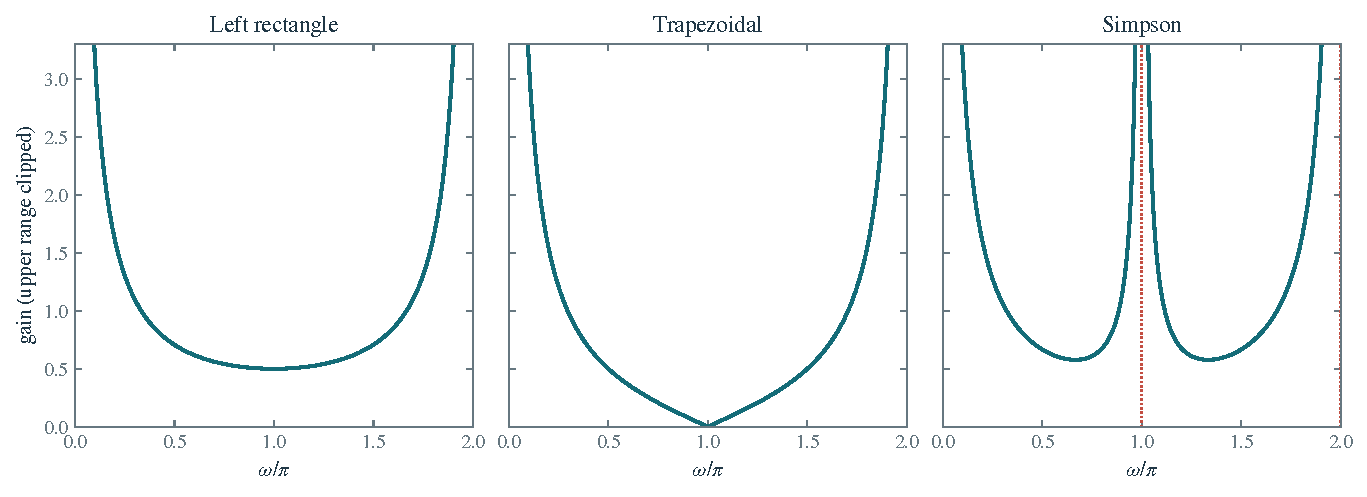
\includegraphics[width=\linewidth]{figures/chapter-related-transforms/quadrature-filter-responses/figure.pdf}
\caption{Magnitudes of the rectangle, trapezoidal, and Simpson integration filters for $\Delta=1$. The poles at zero frequency and the additional Simpson pole at the Nyquist frequency are excluded from the plotted grid.}
\label{fig-meth-quadratures-recursive-filter}
\end{figure}
\end{correction}

\begin{correction}{exo-calcul-spline-iir}
\begin{enumerate}
\item Convolving four interval indicators gives
\[
 \beta^3(x)=\begin{cases}
 2/3-|x|^2+|x|^3/2,&|x|\leq1,\\
 (2-|x|)^3/6,&1\leq|x|\leq2,\\
 0,&|x|\geq2.
 \end{cases}
\]
Its only nonzero integer samples are $1/6,2/3,1/6$ at $-1,0,1$.
Thus $D(z)=\Zz(\beta_d^3)(z)=(z+4+z^{-1})/6$.
\item Set $q=\sqrt3-2$ and $A=-6q$. Since $|q|<1$ and
$-6q/(1-q^2)=\sqrt3$, factorization and partial fractions give
\[
 \frac1{D(z)}=\frac{A}{(1-qz^{-1})(1-qz)}
 =\sqrt3\left(\frac1{1-qz^{-1}}+\frac1{1-qz}-1\right).
\]
The causal series converges for $|z|>|q|$, and the anticausal series for
$|z|<1/|q|$. Their common annulus contains the unit circle and defines
the stable inverse. Both denominators have a minus sign.
\item Write $P=2(K-1)$ for the period of the mirror extension. The exact
initial value for the causal pass is
\begin{align*}
 d_0&=\sum_{j=0}^{\infty}q^j u[-j]\\
 &=\frac{u_0+q^{K-1}u_{K-1}
     +\sum_{j=1}^{K-2}(q^j+q^{P-j})u_j}{1-q^P}.
\end{align*}
To obtain it, group the infinite sum by periods of length $P$ and sum the
geometric series. Initialize the anticausal pass $e_{K-1}$ by the same
formula applied to the reversed data. Then compute
\[
 d_k=u_k+qd_{k-1},\qquad e_k=u_k+qe_{k+1},\qquad
 c_k=\sqrt3(d_k+e_k-u_k).
\]
The forward recursion runs from $1$ to $K-1$, and the backward recursion
from $K-2$ down to $0$. Arbitrarily setting their initial values to zero
would change the boundary condition and would not even preserve constant
data. Program~\ref{listing-spline-1} includes the exact initialization.
For $K=1$, use the constant extension, which gives $c_0=u_0$.
\begin{listing}[H]
\PythonCode{listing-spline-1}
\caption{Cubic spline prefiltering with exact mirror initialization and parallel passes.}
\label{listing-spline-1}
\end{listing}
\item The product factorization gives a causal pass $d_k=u_k+qd_{k-1}$
with the same $d_0$, followed by
\[
 c_k=A d_k+q c_{k+1}.
\]
To initialize the backward pass, use mirror symmetry $c_K=c_{K-2}$
and the two equations at $K-1$ and $K-2$. Eliminating $c_{K-2}$ gives
\[
 c_{K-1}=\frac{A}{1-q^2}(d_{K-1}+qd_{K-2}).
\]
This proves Program~\ref{listing-spline-2}. Both constructions solve
\[
 u_0=\frac{4c_0+2c_1}{6},\quad
 u_k=\frac{c_{k-1}+4c_k+c_{k+1}}6,\quad
 u_{K-1}=\frac{2c_{K-2}+4c_{K-1}}6.
\]
The middle formula applies to $1\leq k\leq K-2$. These equations also
provide a direct way to verify the coefficients. The boundary convention
here is mirror extension, distinct from the natural or not-a-knot
conditions in the previous chapter.
\begin{listing}[H]
\PythonCode{listing-spline-2}
\caption{The same mirror-boundary spline prefilter as a cascade.}
\label{listing-spline-2}
\end{listing}
\end{enumerate}
\end{correction}

\begin{correction}{exo-chirp-transform-finis-corps}
Since $a\mapsto g^a$ enumerates the nonzero residues, for $0\leq b<p-1$,
\[
 \wh f(g^{-b})=f(0)+\sum_{a=0}^{p-2}f(g^a)\omega_p^{-g^{a-b}}.
\]
Set $h[a]=f(g^a)$ and $v[a]=\omega_p^{-g^{-a}}$, both indexed modulo
$p-1$. Then $\wh f(g^{-b})=f(0)+(h*v)[b]$. The remaining output is
$\wh f(0)=\sum_x f(x)$. Three length-$(p-1)$ transforms compute the
convolution; the transform of $v$ can be reused for repeated inputs.
The benefit depends on how efficiently this composite length is handled.
Program~\ref{fft-chirp} performs the permutations explicitly and checks
the prime-length and generator assumptions.
\begin{listing}[H]
\PythonCode{fft-chirp}
\caption{Rader's prime-length FFT with explicit input and output permutations.}
\label{fft-chirp}
\end{listing}
Python's three-argument \texttt{pow} computes a modular inverse with an
exponent of $-1$, raising an error when the inverse does not exist.
\begin{listing}[H]
\PythonCode{listing-invmod}
\caption{Exact modular inversion using Python integers.}
\label{listing-invmod}
\end{listing}
\end{correction}

\begin{correction}{exo-calcul-approaches-transfo-frac}
\begin{enumerate}
\item With $x_j=a_0+jh$ and $\xi_k=\xi_0+k\delta$, the rectangle rule gives
\begin{align*}
 \wh f(\xi_k)&\approx h\sum_{j=0}^{N-1}f(x_j)e^{-\imath\xi_k x_j}\\
 &=h e^{-\imath a_0\xi_k}\sum_{j=0}^{N-1}
 \underbrace{f(x_j)e^{-\imath h\xi_0j}}_{\widetilde f[j]}
 e^{-\imath h\delta jk}.
\end{align*}
The inner sum is an $M$-output CZT with $z=e^{\imath h\delta}$.
If $h\delta/(2\pi)=p/q$ in lowest terms, choose $Q\geq N$ a multiple
of $q$ and pad $\widetilde f$ to length $Q$. The required entries of its
DFT have indices $(pQ/q)k\bmod Q$. In particular, $Q=q$ suffices when
$q\geq N$. For $q$ much larger than $N+M$, a chirp convolution of length
at least $N+M-1$ can avoid that large transform. These are equivalent
ways to evaluate the chosen quadrature sum; neither removes its
quadrature error.
\item With $N=2J+1$ endpoint-inclusive samples and $h=a/(N-1)$, Simpson's
rule assigns weights
\[
 (w_0,\ldots,w_{N-1})=\tfrac13(1,4,2,4,2,\ldots,4,1).
\]
Replace $\widetilde f[j]$ by $w_jf(x_j)e^{-\imath h\xi_0j}$ and retain the
outer factor $h e^{-\imath a_0\xi_k}$. Program~\ref{listing-czt-simpson}
uses the unscaled integer weights and puts $1/3$ in the outer factor.
The new spacing $h$ and the final endpoint are essential; they differ
from the rectangle grid.
\begin{listing}[H]
\PythonCode{listing-czt-simpson}
\caption{Fourier-integral quadrature with Simpson weights and physical phases.}
\label{listing-czt-simpson}
\end{listing}
\end{enumerate}
\end{correction}

\begin{correction}{exo-transforme-fourier-fractionionnaire-2d}
For $f\in\CC^{N_1\times N_2}$, the separable transform is
\[
 G_2(f,\alpha)[k,l]=\sum_{n=0}^{N_1-1}\sum_{m=0}^{N_2-1}
 f[n,m]\exp\left(-2\pi\imath\alpha\left(\frac{nk}{N_1}+\frac{ml}{N_2}\right)\right).
\]
Apply the one-dimensional map along each axis. The chirp parameter for an
axis of length $N$ is $e^{+2\pi\imath\alpha/N}$, since the definition
of the CZT already contains a negative exponent. At $\alpha=1$, this
recovers the usual DFT with its negative phase; the opposite sign would
instead give the unnormalized inverse transform.
\begin{listing}[H]
\PythonCode{listing-frft}
\caption{A scaled-frequency Fourier transform with the DFT sign convention.}
\label{listing-frft}
\end{listing}
\begin{listing}[H]
\PythonCode{listing-frft2d}
\caption{A scaled-frequency Fourier transform along both array axes.}
\label{listing-frft2d}
\end{listing}
\end{correction}
